\documentclass[11pt]{article}
\pdfinfoomitdate=1\pdftrailerid{}
\usepackage[letterpaper,margin=.7in,headheight=15pt,headsep=18pt,footskip=24pt]{geometry}
\usepackage[T1]{fontenc}\usepackage{lmodern,amsmath,amssymb,array,booktabs,fancyhdr,hyperref,tikz,pifont}
\usetikzlibrary{calc}
\usepackage{enumitem}\setlist[itemize]{topsep=2pt,itemsep=1pt,parsep=0pt,partopsep=0pt}
\renewcommand{\familydefault}{\sfdefault}\setlength{\parindent}{0pt}\setlength{\parskip}{6pt}
\pagestyle{fancy}\fancyhf{}\fancyhead[L]{\small Week NN / Graceful labels / Facilitator guide}
\fancyfoot[L]{\scriptsize Bellingham Math Circle / Week NN / FNN-FAC-v1}\fancyfoot[R]{\thepage}
\renewcommand{\headrulewidth}{0.4pt}
\newcommand{\head}[1]{\par\textbf{\large #1}\par}
\newcommand{\sub}[1]{\par\textbf{#1}\par}
\newcommand{\yes}{\ding{51}}\newcommand{\no}{\ding{55}}
\hypersetup{hidelinks}
\begin{document}
\head{Mathematical overview: the longest link and a climbing count}
\textbf{The rule.} A network with $m$ links is labelled (``graceful'' in the literature) when its dots carry different whole numbers from $0$ to $m$ and the differences along the links are exactly $1,\dots,m$, each once. On the K--1 pages a label is a tower's height, the one empty dot is $0$, and ``how many cubes taller'' is the difference. A tree has one more dot than links and uses every label; a loop leaves exactly one label out (the ``left over'' card or tower).

\textbf{The longest link joins $0$ and $m$.} A difference of $m$ arises only as $m-0$. So every labelling uses $0$ and $m$ on two joined dots: the tallest tower stands beside the empty dot, a star's middle is $0$ or $m$, and neither is ever left over. This explains K--1 Problems 5 and 8, Grades 2--3 Problem 4, and why the tallest tower is never left over in K--1 Problems 6--7.

\textbf{Flipping.} Replacing each label $x$ by $m-x$ keeps every difference, so labellings pair up: middle $0$ with middle $m$, left-over $r$ with left-over $m-r$.

\textbf{Paths, stars and caterpillars always work.} Along a path, $0,m,1,m-1,2,\dots$ gives differences $m,m-1,\dots,1$: the low labels climb by one and the high ones fall by one, so each gap is one shorter than the last. A star takes $0$ in the middle. Run along the spine, the same zigzag labels every caterpillar, a tree that becomes a path when its end dots are removed (Grades 4--5 Problem 9).

\textbf{Theorem (loops; Rosa 1967).} A loop with $n$ links can be labelled exactly when $n$ leaves remainder $0$ or $3$ on division by $4$: $3,4,7,8,11,12,\dots$ but not $5,6,9,10,\dots$. \emph{Why not:} walk once round the loop. Each link is a climb or a fall by its number and you end on your starting label, so climbs and falls have equal totals and $1+2+\dots+n=n(n+1)/2$ is even; for $5$ and $6$ links it is $15$ or $21$. Equivalently, each odd link switches the label between odd and even, a trip home switches an even number of times, and $1$--$5$ and $1$--$6$ each contain three odd numbers. When $1+\dots+m$ is odd, the same count rules out any network in one piece whose dots each touch an even number of links, since it has a walk using every link once and coming home (Week~10's bridges); with several pieces, walk each piece in turn. \emph{Why yes:} Rosa constructed labellings, for example the zigzag that skips one high label, $3k$ when $n=4k$ and $3k+2$ when $n=4k+3$. Each link is one shorter than the last except at the skip, where it is two shorter; the one length jumped over equals the last label, which the closing link back to $0$ supplies (loop of $8$: $0,8,1,7,2,5,3,4$ gives links $8,7,6,5,3,2,1$, then $4-0=4$; our script checked every such loop up to $1000$ links). The climbing count alone never shows that a loop \emph{can} be labelled.

\textbf{Theorem (every two dots joined; rulers).} When every two dots are joined, the labels are marks on a ruler from $0$ to $m$ measuring each length $1,\dots,m$ exactly once. Four dots: $0,1,4,6$ or $0,2,5,6$ only. Five dots: impossible. \emph{Proof 1:} each dot touches four links; round the pentagon and then along the star uses all ten links and comes home, but $1+\dots+10=55$ is odd. \emph{Proof 2:} a distance is odd exactly when one mark is odd and the other even, so $k$ odd marks among five give $k(5-k)\in\{0,4,6\}$ odd distances, never the five odd numbers from $1$ to $10$. Golomb showed that no such ruler exists for six or more dots; neither proof covers six, and the pages do not ask.

\textbf{Conjecture (graceful trees; Ringel and Kotzig, 1960s).} Every tree can be labelled. Gallian's survey (2013 edition) records it as open, with every tree up to 35 dots checked by computer; our script labels every tree shape up to $10$ dots. Online, do not confuse it with ``Ringel's conjecture,'' a weaker relative proved for large trees in 2020 (Montgomery, Pokrovskiy and Sudakov; Keevash and Staden). Check the current survey before telling children nobody knows.

\textbf{Experiments, conjectures and explanations.} A labelling that works proves that network can be labelled; failing to find one is evidence only. Children cross out the loops of $5$ and $6$ after failing, then explain them with the climbing count. ``The tallest tower sits by the empty dot'' begins as a noticed pattern and becomes a one-sentence explanation. ``Every tree can be labelled'' stays a conjecture to test; a tree not yet labelled is not a counterexample.

\textbf{Band map.} \emph{K--1} (counting and comparing towers up to $4$; an adult reads each sentence and writes numbers a child says) places towers and one empty dot on paths, a fork, two stars, a triangle and a square, finds all the ways on the two shortest paths, and decides which middles and left-over towers are possible. \emph{Grades 2--3} (subtraction within $10$; an adult can read the shared rule and scribe the reasons in Problems 4 and 7) label paths up to $11$ dots and two trees, find the middle of a $5$-link star, label or cross out loops of $3$ to $6$ links and then label one of $7$, explain the crossed-out loops as a stretch, and find the four-counter ruler. \emph{Grades 4--5} (subtraction within $12$; sums such as $1+\dots+101$, by pairing; reading alone; written explanations in Problems 2, 4 and 6) justify the path rule, prove the loop rule before the long loops of $7$ and $8$, decide which loops up to $101$ links it rules out, connect rulers to the four- and five-dot networks, and test their own trees against the conjecture.
\head{Preparation, shared launch and pacing}
\textbf{Status.} Prepared for organizer review; unpiloted. Nothing has been tried with real pieces: whether K--1 towers stand on the dots and can be compared there, whether cards stay clear of the link boxes, whether counters sit in the strip squares, and the timings. From the drawings, the printed $2$\,cm cards clear every link box when kept square to the page (about $2$\,mm to spare on the $5$-link loop, the tightest), though a slanted card on the $5$- and $6$-link loops can touch a box corner; a $2$\,cm snap cube clears every K--1 box at any angle.

\textbf{Printing.} Everything is US Letter, single-sided, at 100\% (Actual Size); check the $50$\,mm bar on each materials page with a ruler. \emph{Packets:} one per child, nothing cut (K--1 $7$ pages, Grades 2--3 $7$, Grades 4--5 $9$). The large drawing in each problem is the working board for towers or cards; the small copies are for writing down a way that works, or a cross. \emph{Materials file} (\texttt{materials.pdf}, $3$ landscape pages; card stock helps for page~1):
\begin{itemize}
\item Page 1, \emph{Number cards}: five sets of $0$ to $10$, $2$\,cm square on shared cut lines; each row is one set with its own grey mark, and $6$ and $9$ are underlined. Below them, the \emph{Strip from 0 to 10} ($2.3$\,cm squares) for Grades 4--5 Problem 7. Print $1$: two sets for each of the 2--3 and 4--5 tables, one for the launch.
\item Page 2, \emph{Launch sheet}: the launch network, blank, with $3$\,cm dots. Print $1$.
\item Page 3, \emph{Trees}: the starter trees of Grades 4--5 Problem 9 at card size. Print $2$.
\end{itemize}

\textbf{Materials by table.} Pencils with erasers throughout.
\begin{itemize}
\item \emph{K--1 (two pairs), per pair:} $10$ snap cubes ($2$\,cm) snapped into towers of $1$, $2$, $3$ and $4$, matching each page's tray (pre-built towers prevent two towers of one height). Problem 1 uses the $1$ and $2$; Problems 2, 5 and 6 add the $3$; Problems 3, 4, 7 and 8 use all four.
\item \emph{Grades 2--3 (two pairs), per pair:} one card set; four counters no wider than $2$\,cm ($\tfrac34$-inch counters or single snap cubes) for Problem 8's $0$--$6$ strip on the page ($2.5$\,cm squares); eight at the table.
\item \emph{Grades 4--5 (a pair and a rotating checker):} one card set for the pair and a second so the checker can test a claim without disturbing the board; the materials \emph{Strip from 0 to 10} and five counters of the same kind, reused on the page's $0$--$6$ strip, for Problem 7; the two \emph{Trees} sheets for Problem 9, and blank paper for children's own trees.
\item \emph{Launch:} the \emph{Launch sheet}; towers of $1$, $3$ and $4$ cubes ($8$ more cubes); cards $0$, $1$, $3$ and $4$ from the fifth set.
\end{itemize}
\textbf{Preparation (about 25 minutes with printing, untested).} Cut materials page~1 along its lines into $55$ cards and the strip (about $10$ minutes), and keep each set together by its grey mark. Snap $28$ cubes into the two K--1 tray sets and the launch towers, and count out the counters.

\textbf{Staffing.} \emph{K--1 (parent volunteer):} read each problem sentence aloud while pointing to the tray. The children choose where towers go, stand two towers side by side to compare them, and decide. Writing numbers on the small boards for a child who says them is ordinary support; choosing where towers go is not, and is a signal to go back to a shorter path. Watch for two empty dots: the rule allows exactly one. \emph{Grades 2--3 (mathematician):} after the launch, the labelling problems run independently in pairs, one child placing cards and the other writing each link number. The adult is needed when children cross out a loop (``How do you know?'') and for Problem 7. \emph{Grades 4--5 (organizer):} the third child checks each link number and that none repeats, rotating. The adult joins the explanations in Problems 2, 4, 6, 7 and 8.

\textbf{What to record.} Which problems each table reached; whether partners kept one empty dot and different cards; whether cards and counters fitted the boards; what children said when they crossed out a loop, and explanations in their words. Note separately where an adult chose placements.

\begin{minipage}{\linewidth}
\setlength{\parskip}{6pt}
\textbf{Launch after the movement opening (5 minutes).} Let children hold their own table's towers or cards for a minute. On the \emph{Launch sheet} (materials page 2), a triangle with a tail, which is on no page, make the attempt below: leave the tail dot empty, put the $1$-tower on the corner joined to it, and the $3$ and $4$ on the other two corners. Stand the $3$ beside the $1$: two cubes taller, so write $2$ in that box. Let children measure the other three links: $1$, $3$ and $1$. Then say the goal once: ``There are four links, so we want the link numbers $1$, $2$, $3$ and $4$, each once. We have two 1s and no 4, so this one does not work yet.'' Swap the towers for cards $0,1,3,4$ to show the older tables the same thing with differences. Do not repair the attempt; it shows no answer from any page. Do not use the ticked example from the Grades 2--3 and 4--5 pages: it is one of K--1 Problem 1's answers.
\begin{center}
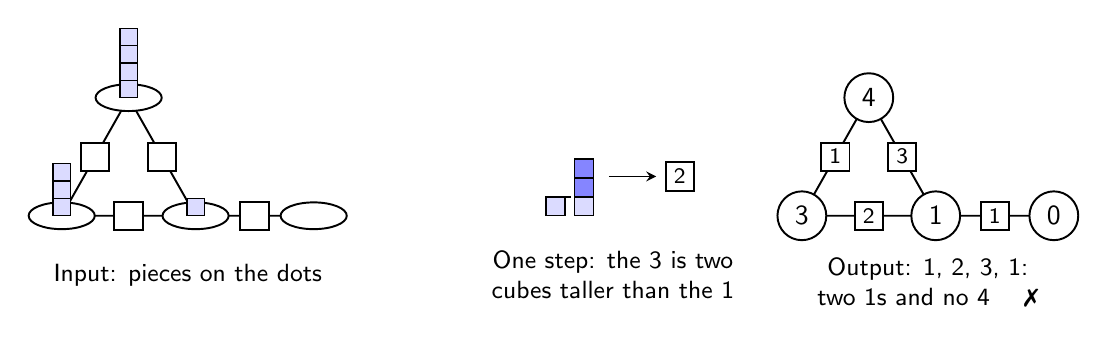
\begin{tikzpicture}[x=1cm,y=1cm,line width=0.7pt]
\tikzset{dot/.style={draw,fill=white,circle,minimum size=0.62cm,inner sep=0pt},
  bx/.style={draw,fill=white,minimum size=0.36cm,inner sep=0pt,font=\footnotesize},
  cube/.style={draw,fill=blue!14,line width=0.5pt}, xcube/.style={draw,fill=blue!48,line width=0.5pt}}
\newcommand{\paw}[9]{% shift x, labels top bl br tail, boxes tl lr tr tail
  \begin{scope}[xshift=#1cm]
  \coordinate (T) at (0,1.5); \coordinate (L) at (-0.85,0); \coordinate (R) at (0.85,0); \coordinate (E) at (2.35,0);
  \draw (T)--(L)--(R)--(T) (R)--(E);
  \node[bx] at ($(T)!0.5!(L)$) {#6}; \node[bx] at ($(L)!0.5!(R)$) {#7}; \node[bx] at ($(T)!0.5!(R)$) {#8}; \node[bx] at ($(R)!0.5!(E)$) {#9};
  \node[dot] at (T) {#2}; \node[dot] at (L) {#3}; \node[dot] at (R) {#4}; \node[dot] at (E) {#5};
  \end{scope}}
% panel 1: towers placed (top 4, lower left 3, lower right 1, tail empty)
\draw (0,1.5)--(-0.85,0)--(0.85,0)--(0,1.5) (0.85,0)--(2.35,0);
\foreach \p in {{(-0.425,0.75)},{(0,0)},{(0.425,0.75)},{(1.6,0)}} {\node[bx] at \p {};}
\foreach \x/\y in {0/1.5,-0.85/0,0.85/0,2.35/0} {\draw[fill=white] (\x,\y) ellipse (0.42 and 0.17);}
\foreach \k in {0,1,2,3} {\draw[cube] (-0.11,1.5+0.22*\k) rectangle (0.11,1.72+0.22*\k);}
\foreach \k in {0,1,2} {\draw[cube] (-0.96,0.22*\k) rectangle (-0.74,0.22+0.22*\k);}
\foreach \k in {0} {\draw[cube] (0.74,0.22*\k) rectangle (0.96,0.22+0.22*\k);}
\node[font=\small] at (0.75,-0.75) {Input: pieces on the dots};
% panel 2: one link measured
\begin{scope}[xshift=5.6cm]
\foreach \k in {0} {\draw[cube] (-0.3,0.24*\k) rectangle (-0.06,0.24+0.24*\k);}
\foreach \k in {0} {\draw[cube] (0.06,0.24*\k) rectangle (0.3,0.24+0.24*\k);}
\foreach \k in {1,2} {\draw[xcube] (0.06,0.24*\k) rectangle (0.3,0.24+0.24*\k);}
\draw[dashed,line width=0.5pt] (-0.3,0.24)--(0.3,0.24);
\draw[->,>=stealth,line width=0.6pt] (0.5,0.5)--(1.1,0.5);
\node[draw,fill=white,minimum size=0.36cm,inner sep=0pt,font=\footnotesize] at (1.4,0.5) {2};
\node[font=\small,align=center] at (0.55,-0.75) {One step: the 3 is two\\cubes taller than the 1};
\end{scope}
% panel 3: written record
\paw{9.4}{4}{3}{1}{0}{1}{2}{3}{1}
\node[font=\small,align=center] at (10.15,-0.85) {Output: 1, 2, 3, 1:\\two 1s and no 4 \quad\no};
\end{tikzpicture}
\end{center}
\end{minipage}

\textbf{A first visit.} After five minutes of running and the five-minute launch, the tables have $35$--$40$ minutes; close with each table showing one network it labelled and one it crossed out, with its reason. Finishing every page is not the goal. \emph{K--1:} Problems 1 and 2 (pages 1--2), then Problem 5 (page 4); Problem 3 if time remains. Save Problem 4 and the loops and middles of Problems 6--8 for a return visit. \emph{Grades 2--3:} Problems 1, 3, 4 and 5 (pages 1, 3--5). Continue with Problem 6 and then Problem 7 with the adult; Problem 2 suits a child who has noticed the zigzag; Problem 8 opens the ruler direction for a quick pair or a return visit. \emph{Grades 4--5:} Problems 1--4 (pages 1--4), then Problem 6. Problem 5's long loops, the rulers and complete networks of Problems 7--8 and the trees of Problem 9 make a full return visit.

\textbf{Hints only when useful.} Ask questions, not steps: ``Which link numbers are missing, and which appear twice?'' When a pair is close: ``Which two pieces could swap to fix the repeated number?'' When a pair wants to cross something out, ask what they tried and whether they are sure; a reason can wait for the explanation problems. Keep ``Which two numbers must be at the ends of the longest link?'' as a last resort for a pair stuck after several tries: it hands over the overview's central fact.

\head{Grades K--1: towers and one empty dot}
Below, $0$ is the empty dot and other numbers are tower heights, listed along a path from the left. Plain-words key for the whole packet: \emph{the tallest tower always stands next to the empty dot.} Mirror images (the same towers read from the other end) count as different ways unless the children decide otherwise; either choice is fine if they say which they use.

\sub{Problem 1, page 1: path of 3 dots, towers 1 and 2}
Exactly $4$ ways: $1$-$0$-$2$, $2$-$0$-$1$, $0$-$2$-$1$, $1$-$2$-$0$ (two ways and their mirror images). Complete: a link of $2$ needs the $2$-tower beside the empty dot, and the $1$-tower then goes on the far side of either one. Ask ``How do you know you have found them all?'' Hint: ``Which tower has to stand next to the empty dot?''

\sub{Problem 2, page 2: path of 4 dots, towers 1, 2, 3}
Exactly $4$ ways: $0$-$3$-$1$-$2$, $3$-$0$-$2$-$1$ and their mirror images $2$-$1$-$3$-$0$, $1$-$2$-$0$-$3$. Complete: the $3$-tower stands beside the empty dot. If those two take the middle pair of dots, the end towers make links $1,1$ or $2,2$; so they sit at one end, and only one order of the other two towers works each way round. Hint: ``Can the $3$ and the empty dot both be in the middle?''

\sub{Problems 3 and 4, page 3: path of 5 dots and the fork}
Path: $8$ ways, for example $0$-$4$-$1$-$3$-$2$ (links $4,3,2,1$): empty, tallest, shortest, next tallest, \dots. Fork: $12$ ways, for example empty dot on the left end, $4$ on the dot where the path branches, $2$ then $3$ along the rest of the row, $1$ below the branch (links $4,2,1,3$). Hint for both: ``Where can the $4$ go?'' Extension: find a second way.

\sub{Problem 5, page 4: star with 3 links}
Finish the small pictures with middle $0$ (empty) and middle $3$; the other three pieces go round the outside in any order. Cross out middles $1$ and $2$. A child's reason: the $3$-link needs the $3$-tower and the empty dot together, and every link touches the middle, so one of them must be the middle. With $1$ in the middle the outside pieces $0,2,3$ make links $1,1,2$; with $2$, links $2,1,1$. Hint: ``Which two have to be joined to make the $3$?''

\sub{Problem 6, page 5: triangle, towers 1, 2, 3}
Circle $1$ and $2$. Empty, $1$, $3$ gives links $1,2,3$ with the $2$ left over; empty, $2$, $3$ gives $2,1,3$ with the $1$ left over. The $3$ is never left over, since nothing else makes a $3$-link. Every two dots of a triangle are joined, so once the three pieces are right, any placement works. Hint: ``Which two pieces could make the $3$? Can the $3$-tower stay in the tray?''

\sub{Problem 7, page 6: square, towers 1, 2, 3, 4}
Circle $1$ and $3$. Going round: empty, $2$, $1$, $4$ (links $2,1,3,4$) leaves the $3$; empty, $4$, $2$, $3$ (links $4,2,1,3$) leaves the $1$. The $4$ must be used. If the $2$ is left over, the empty dot and the $4$ are joined, the $1$ and $3$ are joined to each other, and the two remaining links measure $1,1$ or $3,3$. ``How do you know the $2$ cannot be left over?'' is a good question for a child who circled only $1$ and $3$. Hint: ``Where must the $4$-tower stand?''

\sub{Problem 8, page 7: star with 4 links}
The $4$-tower, or no tower: the middle can also be the empty dot. Either way the other four pieces go outside in any order ($24$ ways each). The reason is Problem~5's. Because the question says ``which towers,'' children may miss the empty middle; ask ``Could the middle be the empty dot?''

\head{Grades 2--3: cards, loops and a ruler}
\sub{Problem 1, page 1: paths of 4, 5 and 6 dots}
From the left: $0,3,1,2$; \ $0,4,1,3,2$; \ $0,5,1,4,2,3$. There are $4$, $8$ and $24$ labellings in all. Many children find the zigzag (smallest, largest, next smallest, next largest). Hint: ``Where can the biggest card go?''

\sub{Problem 2, page 2: path of 11 dots}
$0,10,1,9,2,8,3,7,4,6,5$ along the snake from the top left ($648$ labellings in all). Hint: ``What did your paths in Problem 1 have in common?''

\sub{Problem 3, page 3: two trees}
Fork: $0$ on the left end, $4$ on the branch dot, $2$ then $3$ along the row, $1$ below (links $4,2,1,3$; $12$ in all). Two joined middles with two outer dots each: one middle $0$ with outer dots $1$ and $4$, the other middle $5$ with outer dots $2$ and $3$ (links $1,4,5,3,2$; $48$ in all). Hint: ``Which card must be next to the $0$?''

\sub{Problem 4, page 4: middle of the 5-link star}
Only $0$ or $5$, each with the other cards outside in any order. A link of $5$ can only be made by $0$ and $5$, and every link touches the middle, so one of them is the middle. For the other cards the explanation is the same each time: with $2$ in the middle, a $5$-link would need a $7$, which is not a card. Hint: ``Which two cards can make the link of $5$?''

\sub{Problem 5, page 5: loops of 3, 4, 5 and 6 links}
Label the loops of $3$ and $4$; cross out $5$ and $6$. Going round: $0,1,3$ or $0,2,3$ (the $2$ or the $1$ left over); $0,2,1,4$ or $0,4,2,3$ (the $3$ or the $1$ left over). The loops of $5$ and $6$ have no labelling (a computer tried every arrangement); children cross them out after many failures, which is evidence, and Problem 7 asks for the reason. If a child is stuck on the $5$-loop, ask ``Which card are you leaving out? Have you tried leaving out a different one?'' and later ``Do you think it can be done?''

\sub{Problem 6, page 6: loop of 7 links}
For example $0,7,1,6,2,4,3$ going round: the path zigzag with the $5$ left out ($168$ labellings in all). Only about $1$ in $240$ arrangements of the cards works, so random trying is slow. Hint: ``Which two cards must be neighbours?'' Only as a last resort, since it hands over the construction: ``Could you start like a path, $0,7,1,6,\dots$, and leave out one card?''

\sub{Problem 7, page 6: why the crossed-out loops fail}
The climbing count from the overview. A third-grade route: walk a finger round the loop; each link is a step up or a step down by its number, and you come back to the same card, so the ups add up to the same as the downs. All the link numbers together then make an even total, but $1+2+3+4+5=15$ and $1+2+\dots+6=21$ are odd. On a labelled square the climbs and falls are $1,4$ and $2,3$ in some order, and $1+4=2+3$. A held prompt: ``You came back to where you started. What do you know about the ups and the downs?'' Follow-ups: ``Does this show that the $3$- and $4$-loops can be labelled?'' (no; it only fails to rule them out) and ``Which loop is the next one it rules out?'' ($9$ and $10$). This is the stretch problem of the packet; a construction plus ``we tried a lot'' is a fine place to stop.

\sub{Problem 8, page 7: four counters on the strip from 0 to 6}
Counters at $0,1,4,6$ or $0,2,5,6$ (mirror images). Complete: a distance of $5$ needs a counter at $1$ (with $6$) or at $5$ (with $0$). With $1$, the distances so far are $1,5,6$, and the last counter must make $2,3,4$: only $4$ does ($2$ repeats $1$, $3$ makes two 3s, $5$ repeats $1$). With $5$, the mirror image gives $2$. Hint: ``Which squares could make the distance $5$?'' Extension: put $0,1,4,6$ on four dots that are all joined to each other, and check the six links (Grades 4--5 Problem 8).

\head{Grades 4--5: rules, proofs, rulers and trees}
\sub{Problem 1, page 1}
Path of 6 from the left: $0,5,1,4,2,3$ ($24$ labellings). Two joined middles: as in Grades 2--3 Problem 3. Hint: ``Where can the $5$ go?''

\sub{Problem 2, page 2: any path}
$0,10,1,9,\dots,5$ along the snake. The rule $0,m,1,m-1,2,\dots$ uses each label from $0$ to $m$ once, and its gaps are $m,m-1,\dots,1$ because the low labels climb by one while the high labels fall by one. A complete explanation says both why the link numbers are all different and why they run from $1$ to $m$. Hint: ``Read the link numbers along your path. What happens from one link to the next?'' Other rules exist ($648$ labellings for $11$ dots). Extension: does the idea work for a star, or for a path with extra dots hanging off it (the caterpillar of Problem 9)?

\sub{Problem 3, page 3, and Problem 4, page 4: loops and the proof}
Answers as Grades 2--3 Problem 5, and the climbing count of the overview, in either form. Held prompt for Problem 4: ``If you walk round the loop and come back to the start, what do you know about all the ups and all the downs?'' A child who argues with odd and even numbers has an equally good proof. Ask whether the argument shows that the $3$- and $4$-loops \emph{can} be labelled; it does not.

\sub{Problem 5, page 5: loops of 7 and 8 links}
Both can be labelled. The climbing count allows them ($28$ and $36$ are even), and constructions settle them: $0,7,1,6,2,4,3$ and $0,8,1,7,2,5,3,4$ going round ($168$ and $384$ labellings; about $1$ in $240$ and $1$ in $945$ random arrangements). Hint: ``Which two cards must be neighbours?'' Only as a last resort, since it hands over the construction: ``What happens if you go round the loop with a path labelling? Which link goes wrong, and what if you leave out a different card?''

\sub{Problem 6, page 6: 9, 10, 11, 12, 100 and 101 links}
The proof rules out $9$, $10$ and $101$: $1+\dots+9=45$, $1+\dots+10=55$ and $1+\dots+101=5151$ are odd. For $11$, $12$ and $100$ the totals $66$, $78$ and $5050$ are even, so the proof says nothing, and in fact they can be labelled: $0,11,1,10,2,9,3,7,4,6,5$ and $0,12,1,11,2,10,3,8,4,7,5,6$, and for $100$ the same zigzag skipping $75$. So ``I cannot show it'' is the honest answer for those three. Pairing $1+100$, $2+99$, \dots\ gives $50\times101$ quickly. Hints: ``Which of these totals do you already know?'' ``Is there a quick way to add $1$ to $100$?'' Extension: which numbers of links does the proof rule out? (Those leaving remainder $1$ or $2$ on division by $4$.)

\sub{Problem 7, page 7: rulers}
Four counters: $0,1,4,6$ or $0,2,5,6$, as Grades 2--3 Problem 8. Five counters from $0$ to $10$: impossible. A child's case argument: a distance of $9$ needs a counter at $1$ or $9$; by mirror image say $1$. A distance of $8$ then needs a counter at $8$, since $2$ would make a second $1$ and $9$ a second $9$. Now $0,1,8,10$ give $1,2,7,8,9,10$, and the last counter must make $3,4,5,6$; each empty square repeats a distance (try $2$ to $7$ and $9$). A shortcut: a counter at $x$ between $2$ and $7$ adds distances $x$, $x-1$, $8-x$ and $10-x$, which always total $17$, but $3+4+5+6=18$. The odd-and-even proof of the overview is the adult's version. Hint for five counters: ``With counters on $0$ and $10$, where could a distance of $9$ come from?'' Five counters go on the materials \emph{Strip from 0 to 10} (page 1); the page's $0$--$10$ strips ($1.7$\,cm squares) are too small for counters and serve for writing down tries.

\sub{Problem 8, page 8: four and five dots, all joined}
Four dots: $0,1,4,6$ placed anywhere (all $24$ placements work, since every two dots are joined), or $0,2,5,6$. Five dots: impossible, and Problem 7 is the reason, since the labels would be five counters from $0$ to $10$ with every distance once. A second proof reuses Problem 4: trace the pentagon and then the star, a trip using every link once that comes home, while $1+\dots+10=55$ is odd. Hints: ``How is this like Problem 7?'' ``Can you travel along every link once and come back?''

\sub{Problem 9, page 9: trees}
The spider: middle $0$; one leg $6$ then $1$, another $4$ then $3$, the third $2$ then $5$ (links $6,5$; $4,1$; $2,3$; $60$ labellings in all). The caterpillar: left end $0$, the dot with four neighbours $7$, its upper and lower dots $1$ and $2$, the next dot along $3$ with $6$ below it, the last dot $5$ with $4$ below it (links $7,6,5,4,3,2,1$; $144$ in all). That is the path zigzag run along the spine, and children can turn it into a rule for every caterpillar: $0$ on the end dot of a longest path and the top card on its neighbour; that dot's other neighbours get the next low cards, ending with the next dot along the spine; that dot's new neighbours get the next high cards, again ending on the spine; and so on. Each new link is one shorter than the last. The printed trees' dots are too small for cards: lay cards on the materials \emph{Trees} sheet (page 3), or write numbers on the page. Hint: ``Which card must be next to the $0$?'' The spider is the smallest tree that is not a caterpillar, so the rule does not reach it. ``Can you find a tree that cannot be labelled?'' No one had by the 2013 survey (see the overview), and every tree with up to $10$ dots was checked here. A child who cannot label a tree has a candidate, not a counterexample: the table can try it together, and the adult can ask which trees were hardest and why.

\head{Sources and use}
Alexander Rosa, ``On certain valuations of the vertices of a graph,'' in \emph{Theory of Graphs} (International Symposium, Rome, 1966), Gordon and Breach, 1967, pp.~349--355: the loop theorem. Solomon W. Golomb, ``How to number a graph,'' in \emph{Graph Theory and Computing}, ed. R.~C. Read, Academic Press, 1972: complete networks and rulers. Joseph A. Gallian, ``A Dynamic Survey of Graph Labeling,'' \emph{Electronic Journal of Combinatorics} DS6, 16th ed. (2013): \S2.1 pp.~7 and~9 (trees; the conjecture open; trees up to 35 dots checked), \S2.2 p.~9 (cycles, Rosa), \S2.4 pp.~16 and~18 (complete graphs, Golomb rulers). JRMF, \emph{Graceful Gourds} (web page) and its \emph{Graceful Graphs Festival Guide}, pp.~2--3, a model of a short rule demonstration (see \texttt{plans/atlas/DESIGN.md}). These come from the theme's outline and were not re-read for this guide; check the current survey before saying the conjecture is open. R.~Montgomery, A.~Pokrovskiy and B.~Sudakov, ``A proof of Ringel's conjecture,'' arXiv:2001.02665 (2020), located for this guide; Keevash and Staden's independent proof is cited from memory. Every count, labelling and impossibility above was recomputed from the final pages by \texttt{check\_guide.py} in this guide's source folder; the zigzag loops up to $1000$ links and the caterpillar rule on random caterpillars are computer checks. Library links: Week~10 (walks over every bridge and odd islands), Week~29 (which lengths rods build on a strip) and Week~55 (cards and sums on a strip).

\end{document}
